\chapter{Emotions and facial analysis}
\label{ch:literature-face}

The human face is a source of information and an important part of communication. Several elements connect this channel of information to emotional states, such as facial expressions and the activity of eyes and head \parencite{akakin2010spatiotemporal}. The analysis of such elements can convey information regarding emotional states, e.g. facial expressions are considered one of the most relevant features that can provide an indication about emotional states \parencite{cowie2001emotion}.

Facial analysis is a promising approach to detecting the emotional state of players unobtrusively and without interruptions \parencite{cohn2014automated}. The use of computer vision for player experience detection is feasible and visual inspection of gaming sessions has shown that the automated analysis of facial expressions is sufficient to infer the emotional state of players \parencite{tan2012feasibility,tan2014inferring}. Automatically detected facial expressions have been correlated with dimensions of game experience \parencite{tan2014correlation} and used to enhance player's experience in online games \parencite{zhou2004real,zhan2008real}. Although automated facial analysis has become mature enough for affective computing, there are several challenges associated with the process. Facial actions are inherently subtle, making them difficult to model, and individual differences in face shape and appearance undermine generalization across subjects \parencite{cohn2014automated}. Schemes such as the Facial Action Coding System (FACS) \parencite{ekman1977facial,cohn2007observer} aim to overcome these challenges through standardizing the measurements of facial expression by defining highly regulated procedural techniques to detect facial Action Units (AU). In the FACS scheme, facial actions/movements are decomposed into 46 different AUs anatomically related to facial muscles. When analyzed in defined contexts, such mapped actions can present a correlation between determined facial features and emotional states, e.g. stress and boredom.

\begin{table}[h!]
\caption{Categorization of facial elements connected with stress and anxiety according to \textcite{giannakakis2017stress}}
\label{table:stress-facial-features}
\begin{tabular}{lll}%
\toprule%
\textbf{Head} & \textbf{Eyes} & \textbf{Mouth} \\
\midrule
Head movement & Blink rate & Mouth shape \\
Skin color & Eyelid response & Lip deformation  \\
Heart rate (facial PPG) & Eye aperture & Lip corner puller \\
& Eyebrow movements & Lip corner depressor \\
& & Lip pressor \\
\midrule
\textbf{Gaze} & \textbf{Pupil} & \\
\midrule
Saccadic eye movements & Pupil size variation &  \\
Gaze spacial distribution & Pupil ratio variation &  \\
Gaze direction & &\\
\bottomrule%
\end{tabular}%
\end{table}

\textcite{giannakakis2017stress} present a literature review focused on facial elements with value for detection of anxiety and stress, including the involvement of eyes (pupil size variations, gaze distribution, blinking rate), mouth (lips deformation, mouth activity) and head (head movement and velocity). Table \ref{table:stress-facial-features} lists all the identified facial elements. There are indications that blinking increases with emotional arousal, including stress and anxiety levels \parencite{dinges2005optical}. Gaze direction, gaze congruency (agreement between eye and head orientation) and the size of the gaze-cuing effect (facilitation of reaction time towards visual clues) are also influenced by the level of anxiety or stress \parencite{staab2014influence}. Similarly, mouth activity is influenced by conditions of stress, particularly lip movement \parencite{dinges2005optical} and asymmetric lip deformation \parencite{metaxas2004image}. Finally, the frequency of mouth openings has been measured as inversely proportional to the stress level under high cognitive load \parencite{liao2005decision}.

Different approaches have been used to connect facial analysis to the emotional states of users. Initiatives include manual or automated face detection, use of machine learning models to map facial features to emotions and so on. The following sections present, in more detail, works related to face detection, including the approach used for analysis and connection to emotional states.

%%%%%%%%%%%%%%%%%%%%%%%%%%%%%%%%%%%%%%%%%%%%%%%%%%%%%%%%%%%%%%%%%%%%%%%%%%%%%%%%%%%%%%%%%%%%%%%%%%%%%%%
\section{Facial analysis based on sensors}
%%%%%%%%%%%%%%%%%%%%%%%%%%%%%%%%%%%%%%%%%%%%%%%%%%%%%%%%%%%%%%%%%%%%%%%%%%%%%%%%%%%%%%%%%%%%%%%%%%%%%%%

The analysis of facial behavior commonly relies on data obtained from physical sensors, e.g. electromyography (EMG), or from the application of visual methods to assess the face, e.g. feature extraction via computer vision \parencite{schrader2017rising}. The approach based on EMG data uses physical sensors attached to subjects to measure the electrical activity of facial muscles, such as the zygomaticus, the orbicularis oculi and the corrugator supercilii muscles (Figure \ref{fig:face-muscles}), associated with smiling, eyelids control and frowning, respectively.

\begin{figure}[h!]
\centering
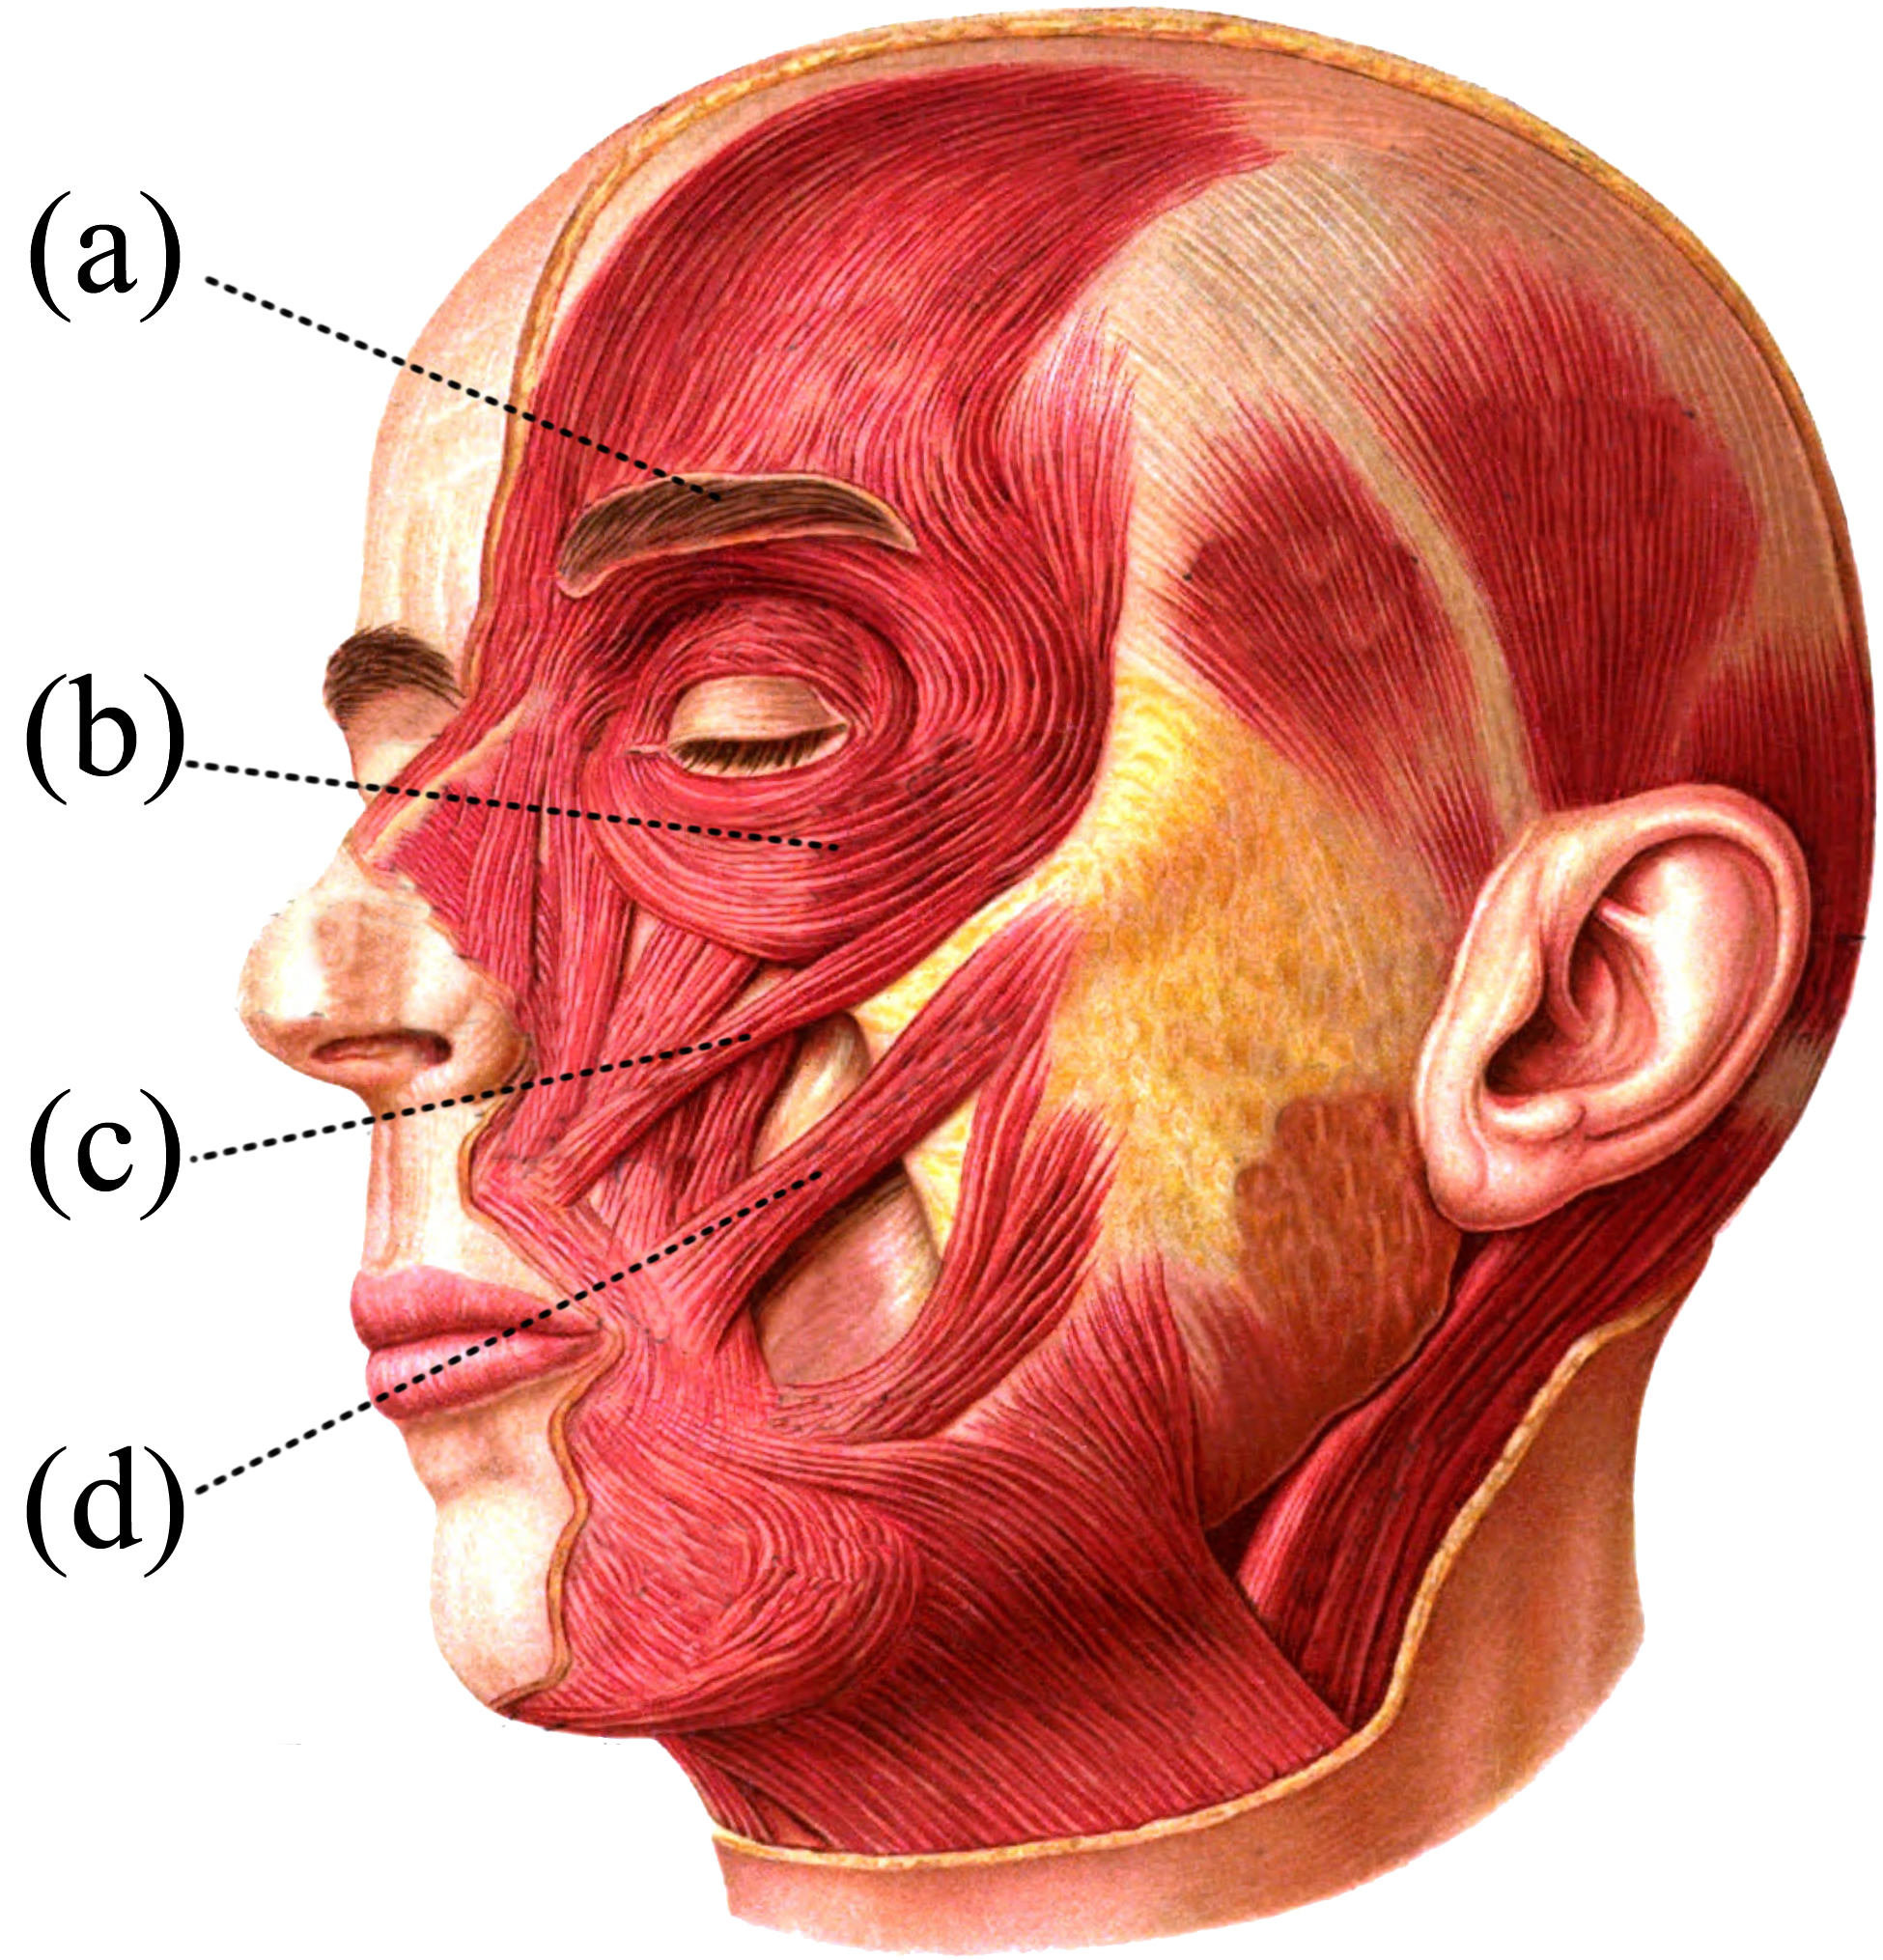
\includegraphics[width=0.8\textwidth]{Content/figures/face-muscles.jpg}
\caption{Facial muscles. (a) Corrugator supercilii. (b) Orbicularis oculi. (c) Zygomaticus minor. (d) Zygomaticus major. Adapted from ``Sobotta's Atlas and Text-book of Human Anatomy", by Dr. Johannes Sobotta (Illustration: K. Hajek and A. Schmitson), 1909. Reproduced from \parencite{sobotta1909wikimedia}.}
\label{fig:face-muscles}
\end{figure}

\textcite{hazlett2006measuring} presents evidence of more frequent corrugator activity when positive game events occur. \textcite{tijs2008dynamic} show that an increased activity of the zygomatic muscle is associated with self-reported positive emotions. Similarly, \textcite{ravaja20051} show that positive and rewarding game events are connected to an increase in zygomatic and orbicularis oculi EMG activity.

Approaches based on EMG are more resilient to variations of lighting conditions and facial occlusion; however, they are obtrusive, since it is necessary to attach physical sensors to the subject's face.

%%%%%%%%%%%%%%%%%%%%%%%%%%%%%%%%%%%%%%%%%%%%%%%%%%%%%%%%%%%%%%%%%%%%%%%%%%%%%%%%%%%%%%%%%%%%%%%%%%%%%%%
\section{Facial analysis based on computer vision}
%%%%%%%%%%%%%%%%%%%%%%%%%%%%%%%%%%%%%%%%%%%%%%%%%%%%%%%%%%%%%%%%%%%%%%%%%%%%%%%%%%%%%%%%%%%%%%%%%%%%%%%

Contrary to the obtrusiveness of EMG-based approaches, the analysis of facial behavior using automated visual methods can be performed remotely and without physical contact. The process usually involves the use of computer vision to perform face detection, the localization of facial features (also known as landmarks or fiducial points) and the classification of such information into facial expressions \parencite{salah2010communication}.

Computer vision systems usually rely on image processing, artificial intelligence, e.g. machine learning, and decision-making techniques to detect and classify objects from images or videos. A class of such objects is the human face, detected and analyzed by a process called facial alignment.

\begin{figure}[h]
    \centering
    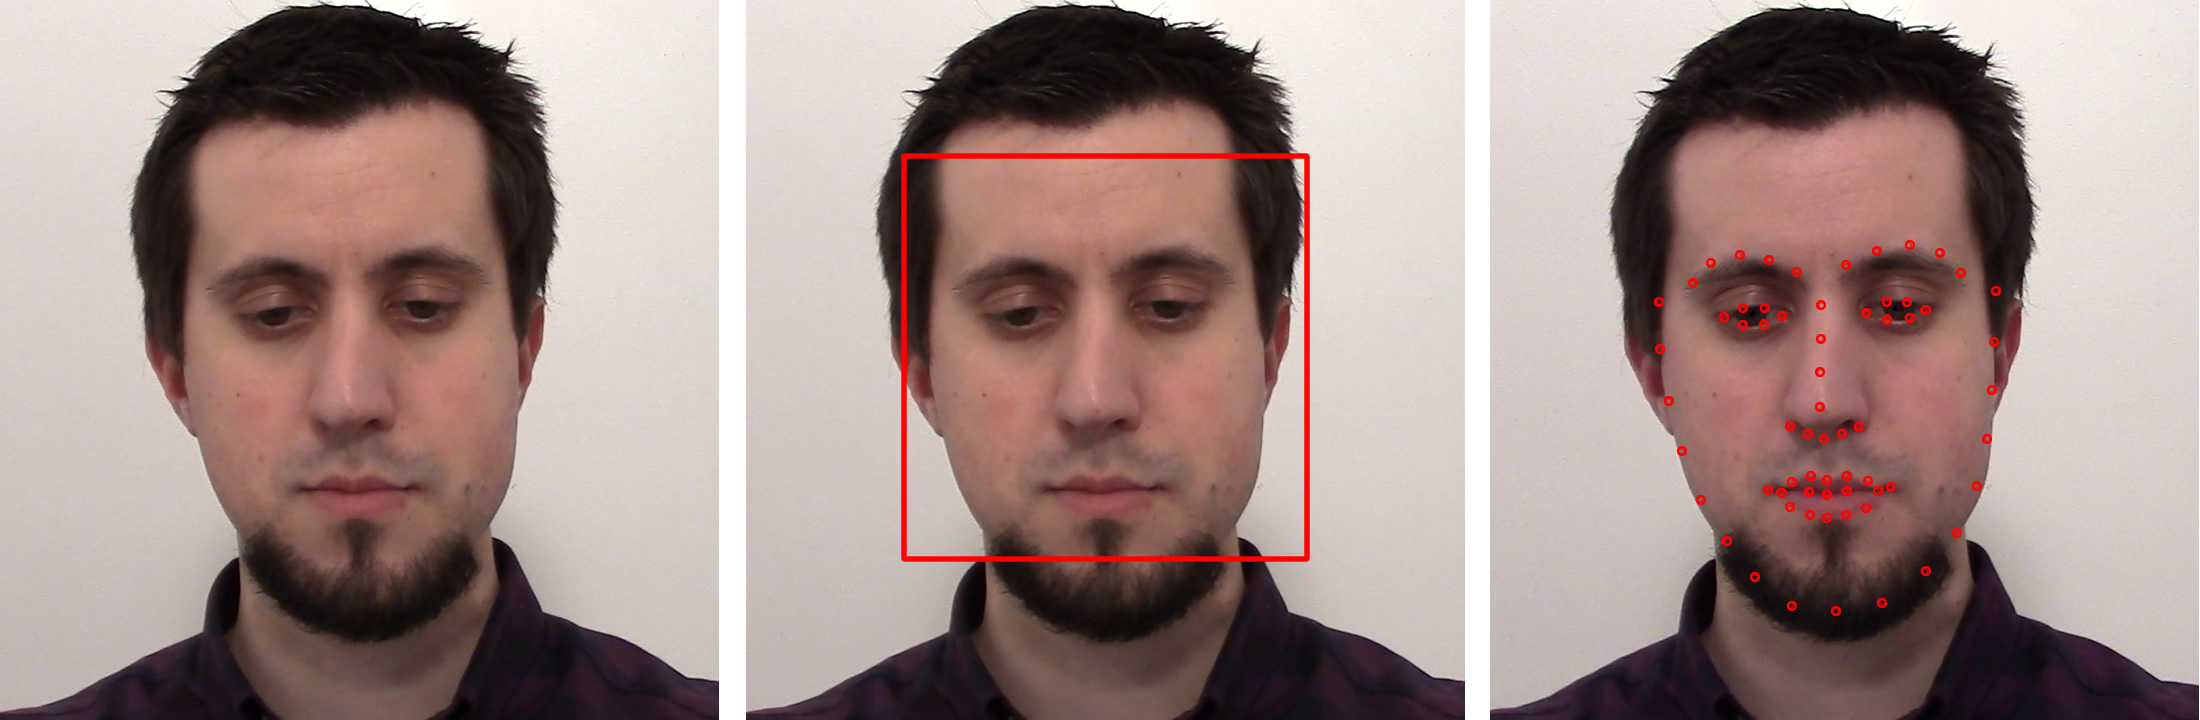
\includegraphics[width=\linewidth]{Content/figures/face-alignment.jpg}
    \caption{Example of face alignment. From left to right: input image, detected face, and aligned face.}
    \label{fig:alignment}
\end{figure}

Facial alignment consists of identifying the position of specific features of the face, e.g. eye and nose, after the face has been detected in an image/video. Figure \ref{fig:alignment} demonstrates the process. This procedure is relevant in many different scenarios, for example, facial/expression recognition and pose estimation. Research has been conducted to create accurate and fast methods that can be used to perform face alignment under an ever growing set of challenging conditions, e.g. face movement combined with different lighting configurations.

Many methods have been proposed and a literature review reveals that two basic approaches are widely used in alignment techniques: constrained local models and cascaded regression methods. Both approaches work on an image of a face contained within a rectangle obtained by a face detection algorithm, such as Viola \& Jones \parencite{viola2004robust}. The following sections describe each one and mention the most relevant techniques for facial alignment that are based on the approach being described.

\subsection{Constrained Local Model}

The Constrained Local Model (CLM) approach consists of locating a set of points on a target image, then applying a constraint to them. The constraint is usually based on a statistical shape model, which is obtained via training in a set of images featuring manually inserted landmarks. Since the shape model is statistical, the position of the points (landmarks) that it describes will always resemble a face, i.e. the proportions of lines and/or the distance between points will not be so different from a human face (at least not different from the ones found in the training set). Figure \ref{fig:clm-models}(a) illustrates the configuration of the shape model with different variations.

\begin{figure}[h]
\centering
  \begin{subfigure}[b]{0.5\textwidth}
    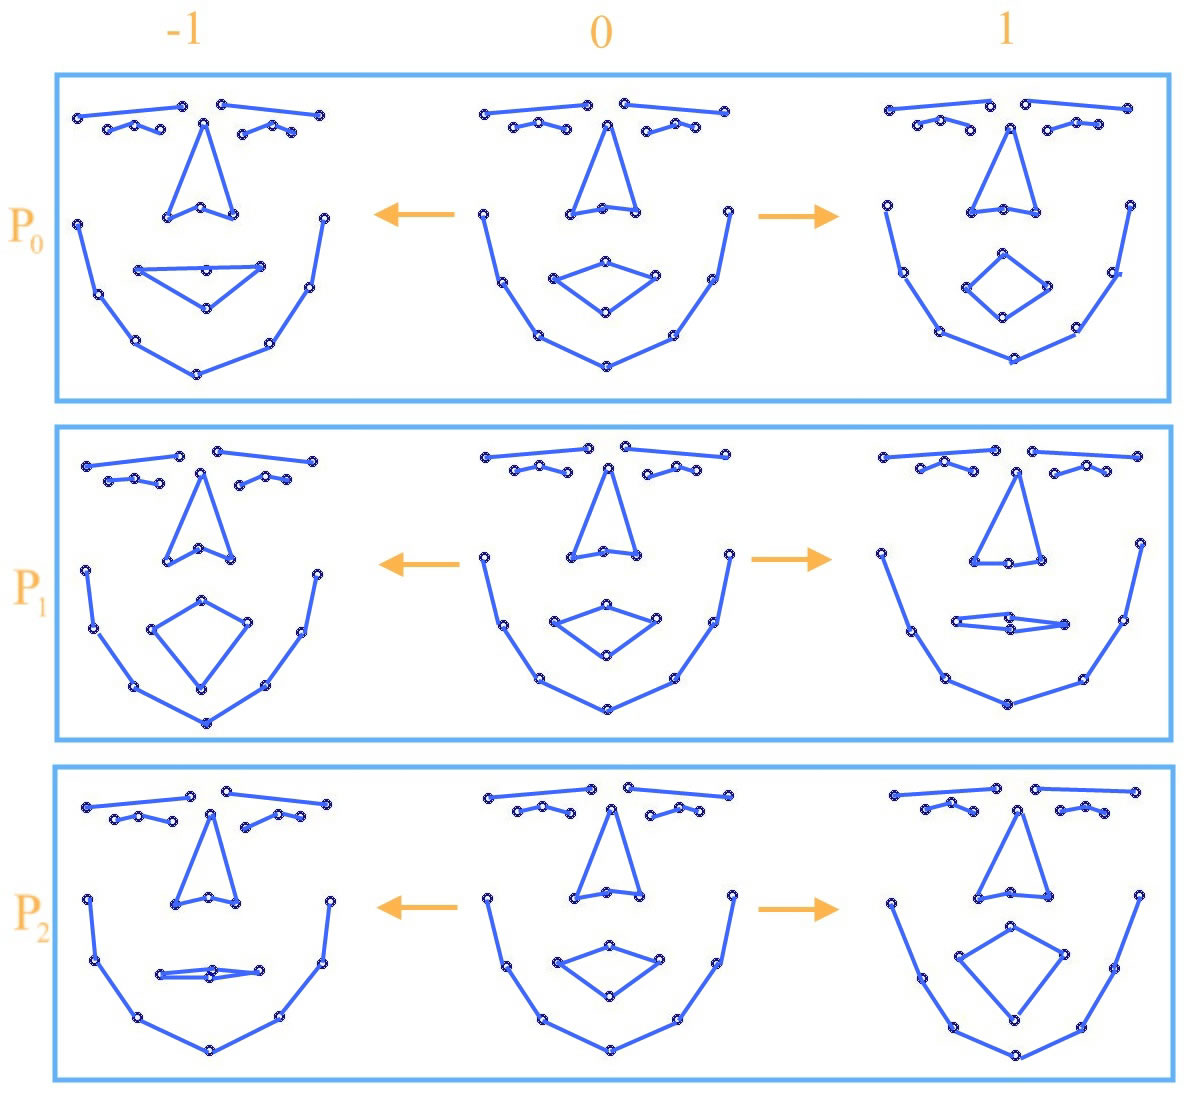
\includegraphics[width=0.95\textwidth]{Content/figures/clm-model-variation.jpg}
    \caption{}
    \label{fig:clm-model-variation}
  \end{subfigure}%
  \begin{subfigure}[b]{0.5\textwidth}
    \centering
    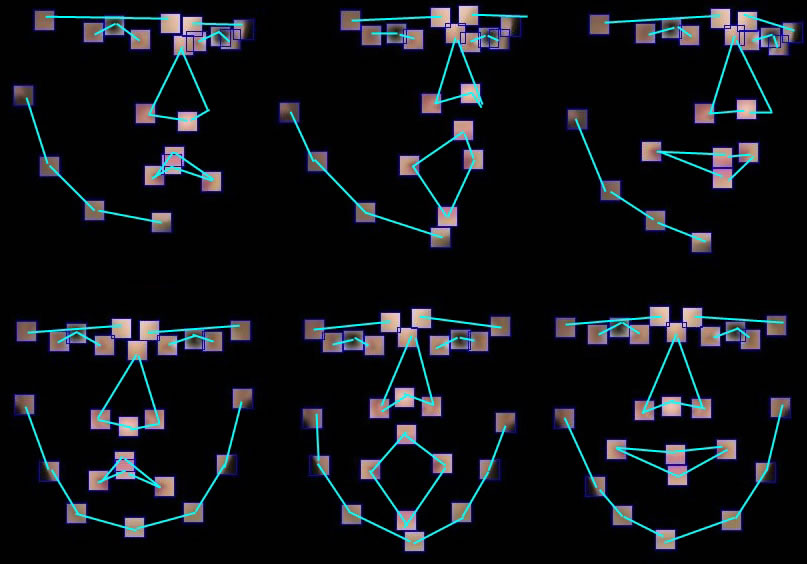
\includegraphics[width=0.95\textwidth]{Content/figures/clm-patches.jpg}
    \caption{}
    \label{fig:clm-patches}
  \end{subfigure}
  \caption{Shape models of CLM. (a) Configuration of the shape models with different variations. (b) Shape models and their respective entries in the texture model. Reproduced from \textcite{yu2010facial}.}
  \label{fig:clm-models}
\end{figure}

In addition to the shape model, there is a texture model that contains a set of patches (images) extracted from the training images by selecting the areas around the inserted landmarks. These patches are used to guide the search procedure in the alignment process, which allows the technique to correctly identify the right model to properly align the face being analyzed. Figure \ref{fig:clm-models}(b) shows different shape models and their respective entries in the texture model.

The process of aligning a face is iterative and starts by sampling points that are placed in the face image according to the current shape estimation of the face. In the first try, this estimation is usually the average face obtained from all training images. The area around the sampled points are extracted and used in a search to locate a set of similar patches in the texture model. The current shape estimation and the texture patches it locates are evaluated according to a cost function. As soon as the shape variation with the minimal cost is found, the process is repeated: new patches are sampled and searched against the texture model, the current estimation is adjusted and so on. Eventually, the cost function will not produce a significantly different value from one iteration to another, which means the current estimation is the best match found.

Figure \ref{fig:clm-evolution} demonstrates the evolution of the technique as it iterates in an image. First the mean shape is placed into the image and the patches are sampled around the (mistakenly) positioned landmarks. As the technique iterates, searched patches progressively induce changes in the current shape model, sampling more accurate patches. Eventually the technique converges to the aligned face.

\begin{figure}[h]
    \centering
    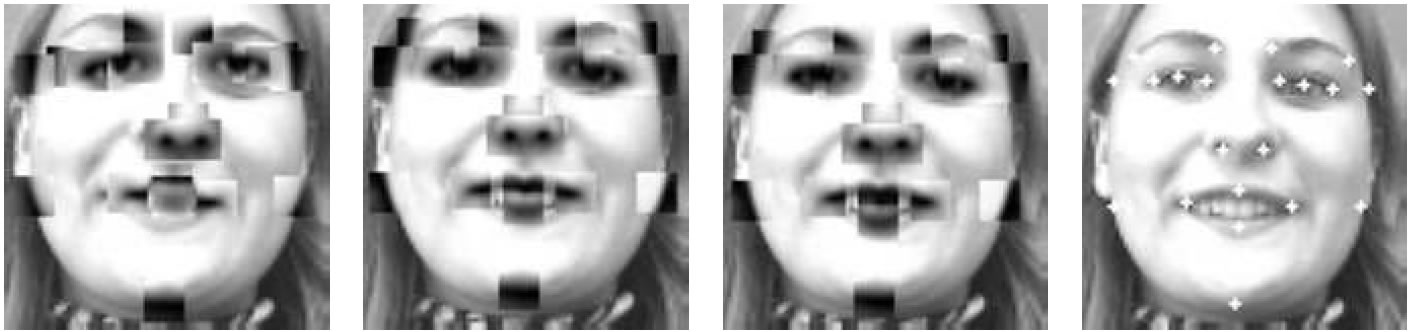
\includegraphics[width=\linewidth]{Content/figures/clm-evolution.jpg}
    \caption{Iteration of CLM during the alignment of an image. Reproduced from \textcite{cristinacce2006feature}.}
    \label{fig:clm-evolution}
\end{figure}

Two techniques that represent the CLM approach are the feature detection and tracking with constrained local models \parencite{cristinacce2006feature} and its 3D variation \parencite{baltruvsaitis20123d}, which uses 3D depth data to improve the process.

\subsection{Cascaded Regression}

The cascaded regression methods approach consists of using an initial guess shape that is progressively refined into the final answer (identification of key features in the image). This refinement is performed in a stage-by-stage manner (cascade) and the result of the current stage is used as the input for the next one. In each stage, the adjustment of the current shape (into the aligned result) is performed by a regression function, learnt via training. Early regressors in the cascade handle large variations in the shape, as opposed to the late ones, which focus on specific details. Each regressor extracts features from the image, which are then worked to produce variations in the current guess shape. The extracted features depend on the current shape and they are commonly referred as shape-indexed features.

The shape-indexed features are differences in pixel intensities. The calculation of a shape-indexed feature involves the selection of a few pixels and the subtraction of their intensities. The way these pixels are selected is usually different for each of the cascaded-regression techniques. Figure \ref{fig:shape-indexed} illustrates an example of the selection of a few pixels for three particular landmarks. The landmark on the top-right (gray circle) highlights the selected pixels that will be used. The difference in intensities among these pixels will define this particular shape-indexed local feature. The shape-indexed local features are used in a decision process in each step (cascade), as illustrated by Figure \ref{fig:regressor-steps}. Usually the initial guess shape is the mean shape of the training set. This guess is used to calculate the current set of shape-indexed features to be extracted, which then guides the variation applied to the current shape. The variation to be applied is usually chosen on the basis of the result of a cost function, which selects a variation that minimizes the distance between the current guess and the supposed aligned face. As the process repeats itself, different shape-indexed features are selected, a new variation is calculated and so on. Eventually, the current shape will converge and will represent the alignment for the face being analyzed (final shape estimation).

\begin{figure}[h]
    \centering
    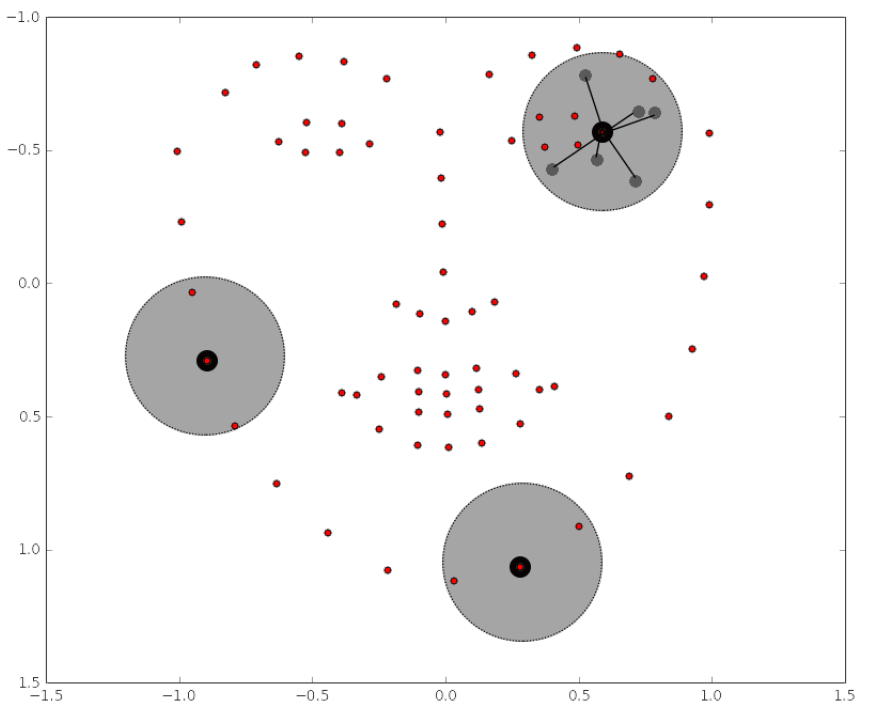
\includegraphics[width=0.6\linewidth]{Content/figures/shape-indexed.png}
    \caption{Pixels used in the calculation of a shape-indexed feature. Reproduced from \textcite{maris2015}.}
    \label{fig:shape-indexed}
\end{figure}

\begin{figure}[h]
    \centering
    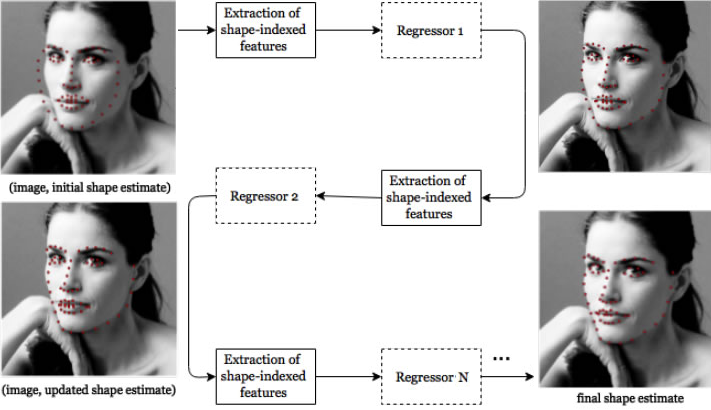
\includegraphics[width=1.0\linewidth]{Content/figures/cascade-explanation.png}
    \caption{Estimation of face shape with regressors in a set of stages. Reproduced from \textcite{maris2015}.}
    \label{fig:regressor-steps}
\end{figure}

Different variations are used to handle the training, the extraction of features and the way the regression is performed. The technique of face alignment with Ensemble of Regression Trees (ERT) \parencite{kazemi2014one}, for instance, estimates the face's landmarks by inputting the regressors with a sparse subset of pixels' intensities, which is calculated with a prior probability on the distance of the pixels.

%The Supervised Descent Method (SDM) \parencite{xiong2013supervised}, on the other hand, extracts SIFT features from the current shape estimation and it converges the shape by solving a series of linear least square problems. The approach via regression of Local Binary Features (LBF) \parencite{ren2014face} proposes the use of a set of local binary features (opposed to a global view of the face) combined with a locality principle for learning and processing such features independently. Finally the face alignment by Explicit Shape Regression (ESR) \parencite{cao2014face} trains the regressors by explicitly minimizing the alignment error over training data, so all facial landmarks are regressed jointly.

%The regressors work by progressively inferring the shape, so the early regressors in the cascade handle large shape variations (ensures robustness) while later regressors focus on the small and subtle variations (ensures accuracy).

%%%%%%%%%%%%%%%%%%%%%%%%%%%%%%%%%%%%%%%%%%%%%%%%%%%%%%%%%%%%%%%%%%%%%%%%%%%%%%%%%%%%%%%%%%%%%%%%%%%%%%%
\section{Facial-based emotion detection}
\label{ch:literature-face-emotion-detection}
%%%%%%%%%%%%%%%%%%%%%%%%%%%%%%%%%%%%%%%%%%%%%%%%%%%%%%%%%%%%%%%%%%%%%%%%%%%%%%%%%%%%%%%%%%%%%%%%%%%%%%%

Facial-based emotion detection techniques try to estimate the emotional state of a subject, based on the analysis of facial features. Works involving such an approach commonly focus on detecting or classifying emotional states, based on the six basic emotions proposed by \textcite{ekman1971constants}, i.e. happiness, surprise, sadness, fear, anger and disgust. Some visual methods rely on manual or automated FACS-based analysis as a standard for categorizing and measuring emotional expressions \parencite{bartlett1999measuring}.

The feasibility of that approach is demonstrated by \textcite{kaiser1994multi}, showing that more AU were reported by manual FACS coders during the analysis of video recordings of subjects playing the stressful part of a game compared to its neutral part. Additionally, authors report lip pull corner and inner/outer brow raise as more frequent AUs during gaming sessions. \textcite{wehrle2000emotion} also support the approach of using an automated, FACS-based facial analysis together with data from game events to provide an appraisal analysis of subjects' emotional state.

\begin{figure}[h]
    \centering
    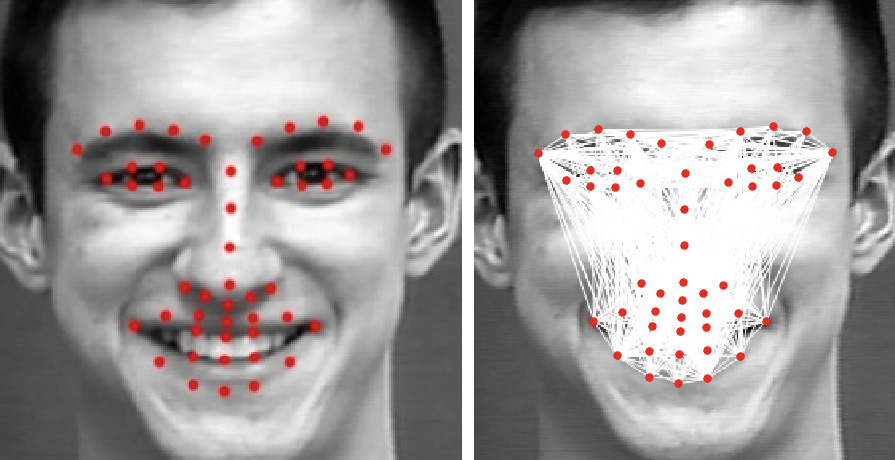
\includegraphics[width=0.75\linewidth]{Content/figures/samara2016sensing-distances.png}
    \caption{Distance-based facial feature descriptors. Left: detected facial landmarks. Right: highlight of the distance between facial landmarks. Reproduced from \textcite{samara2016sensing}.}
    \label{fig:distance-samara}
\end{figure}

Similarly, \textcite{grafsgaard2013automatically} present an experiment where facial expression information is used to investigate emotional states. The experiment consists of an analysis of facial AUs during computer mediated, tutoring sessions among students. Subjects and tutors interact through a tutoring software related to computer programming, while subjects are recorded. After each session, subjects answer a questionnaire related to the measurements of cognitive load and engagement. The recordings are analyzed in an automated way with manual verification of the results. A predictive model is then constructed using the questionnaire's answers and the recording analysis, which results in correlations of facial AU and emotional states. Finally, the authors compare their findings against other research, which differ significantly. For instance, brow lowering has been correlated with confusion in previous work; however, the authors found that it was a positive predictor of student frustration in the context of their experiment.

\textcite{heylen2005facial} also present a similar investigation in a pilot experiment of a tutoring session related to the application of a subcutaneous injection. Students interact with a virtual patient while using a physical haptic device to administrate an injection. The recordings of the students are analyzed by the researchers to make annotations of the expressions based on their own interpretation of the context. The researchers use a compilation of literature components to guide the evaluation of the collected data. As the authors point out, a variety of expressions occur, but most of the time students maintain a neutral facial expression. The annotated features are (ordered from most to less frequent): smile (total 22), raise eyebrows (11), pull down mouth corners (2) and frown (1).

%As opposed to previously mentioned works, our approach consists of using induced boring to stressful mechanics in games to produce variations in the emotional state of participants. Our experiment has a linear progression from a boring to a stressful state that should be perceived by the subjects. We believe such configuration gives our experiment a novel approach for the exploration of facial actions and HR regarding their connection to emotional states, since we can categorize information according to the induced (and theoretically known) emotional states. To the best of our knowledge, this is the first experiment where games with linear boring-to-stressful progression are used to deliberately induce emotional reactions.

In contrast to the previously mentioned works, other initiatives aim to detect emotions based on the analysis of facial landmarks and their distances, movement or angles. \textcite{joho2009exploiting} use facial analysis for affective video summarisation. The authors use an automated face tracking approach to obtain a vector of motion features of certain regions of the face, named Motion Units (MU). MUs are classified by a Bayesian network, which is trained from labeled data. The results indicate a promising correlation between the manually annotated content of the videos and the automatically classified one.

Somewhat similarly \textcite{akakin2010spatiotemporal} detect facial landmarks over consecutive frames of videos, whose trajectories (time series) during head gestures and facial expressions are organized in a spatiotemporal matrix. Discriminative features are extracted from the trajectory matrix and used to train machine learning models, i.e. Adaboost and SVM. Classification accuracy is reported to be around 90\% for the detection of 7 face and head gestures in a dataset composed of 210 videos of 4 subjects. The detection of emotions, however, is limited to only two states, i.e. happiness and sadness.

Finally, \textcite{samara2016sensing} present the sensing of affective states based on the analysis of the distances of facial landmarks. Automated face detection is employed to detect facial landmarks, however no coding scheme is used to identify the detected points. Instead, the authors use the Euclidian distance between facial landmarks, represented as distance vectors, to train a SVM model to detect expressions. Figure \ref{fig:distance-samara} illustrates the process. Detection accuracy is improved by a two-state SVM classification model, which the authors name Hierarchical Parallelised Binary Support Machines. Accuracy rates of about 96\% were achieved on two facial expression datasets. \textcite{samara2016sensing} alse use the Euclidean distance between face points to train a Support Vector Machine (SVM) model to detect expressions. Similarly, \textcite{chang2009emotion} use 12 distances calculated from 14 landmarks to detect fear, love, joy and surprise. \textcite{hammal2007facial} use 5 facial distances calculated from lines in key regions of the face derived from the MPEG-4 animation standard \parencite{abrantes1999mpeg}, e.g. eyebrows, for classification of expressions. \textcite{tang20083d,tang2008line} use up to 30 Euclidean distances between facial landmarks also obtained from MPEG-4 based 3D face models to recognize the 6 universal facial expressions. Similarly \textcite{hupont2013facial} classify the same emotions by using a correlation-based feature selection technique to select the most significant distances and angles of facial points.

The use of facial expressions as a single source of information, however, is contested in the literature. \textcite{blom2014towards} claim that subjects present a neutral face during most of the time of gameplay and frustration is not captured by facial expressions, but by head movements, talking and hand gestures instead. In a similar conclusion, \textcite{shaker2011game} show that head expressivity, i.e. movement and velocity, is an indicator of players' game skills. Additionally, a high frequency level and velocity of head movements is indicative of failing in the game.

%%%%%%%%%%%%%%%%%%%%%%%%%%%%%%%%%%%%%%%%%%%%%%%%%%%%%%%%%%%%%%%%%%%%%%%%%%%%%%%%%%%%%%%%%%%%%%%%%%%%%%%
\section{Summary}
\label{sec:literature-face-summary}
%%%%%%%%%%%%%%%%%%%%%%%%%%%%%%%%%%%%%%%%%%%%%%%%%%%%%%%%%%%%%%%%%%%%%%%%%%%%%%%%%%%%%%%%%%%%%%%%%%%%%%%

Facial analyses based on physical sensors, e.g. EMG, provide continuous monitoring of subjects and are not affected by lighting conditions or pose occlusion by a subject's movement. However, they are obtrusive and the use of sensors increases the user's awareness of being monitored \parencite{yamakoshi2007preliminary,yamaguchi2006evaluation,healey2005detecting}. Approaches based on video analysis, e.g. FACS and computer vision, are less intrusive. Despite the fact that FACS has proven to be a useful and quantitative approach for measuring facial expressions \parencite{bartlett1999measuring}, its manual application is laborious, time-consuming and requires certified coders to inspect the video recordings. The application of FACS also has downsides, including different facial expression decoding caused by misinterpretation in specific cultures \parencite{jack2013culture}.

Facial analyses from visual methods, such as the previously mentioned feature-based approaches relying on computer vision, are quicker and easier to deploy. Automated facial analysis as a mean to detect the emotional state of players has been proven to work at creating emotionally adapted games \parencite{saari2004towards} or tools for unobtrusive game research. When automated facial analysis is used, it is often tested on contexts not related to games, or facial cues are derived from models not designed for the analysis of emotional interactions in games, such as the MPEG-4 standard \parencite{abrantes1999mpeg}. Such a standard specifies representations for 3D facial animations, not emotional interactions in games. Automated facial analysis is also commonly performed on images or videos whose subjects are acting to produce facial expressions, which are likely to be exaggerated in nature and not genuine emotional manifestations. These are artificial reactions that are unlikely to happen in a context involving subjects interacting with real games, where emotional involvement between subject and game is stronger. Another limitation of previous work is the common focus on detecting facial expressions \textit{per se}, e.g. 6 universal facial expressions \parencite{ekman1971constants}, not necessarily detecting isolated facial actions, e.g. frowning, associated with emotional reactions in games. Finally, people are different and elements such as age and familiarity with a game influence the outcome of automated facial analysis of behavioral cues \parencite{asteriadis2012towards}. Furthermore different games might induce different bindings of facial expressions \parencite{tan2014correlation}. Empirical results of manual annotations of facial behavior in gaming sessions have indicated more annotations during stressful than during boring (see Section \ref{sec:experiment1-study1}) or neutral \parencite{kaiser1994multi} parts of games. As a consequence, a more user-tailored contextualization is essential for any study involving facial analysis, particularly involving games.

%Further investigation of such findings using an automated analysis instead of a manual approach is a topic of interest for game researchers and practitioners, who can benefit from improved tools related to facial behavior analysis.

%However previous works commonly focus on analyzing images or videos whose subjects performed facial expressions on guidance. Those are artificial circumstances that do not portrait natural interactions of users and games, for instance. When the analysis is performed on videos of subjects interacting with games, usually the aim is to detect a very specific set of facial expressions, e.g. 6 universal facial expressions, disregarding head movement and subtle changes in facial behavior.

%Such difference in results is expected due to the variational nature of facial expressions among different individuals and contexts, however it underlines the complexity of correlating facial features and emotions
